\subsection{The Multivariate Oxide Composition Model}\label{sec:moc}
\begin{figure}[ht]
    \centering
    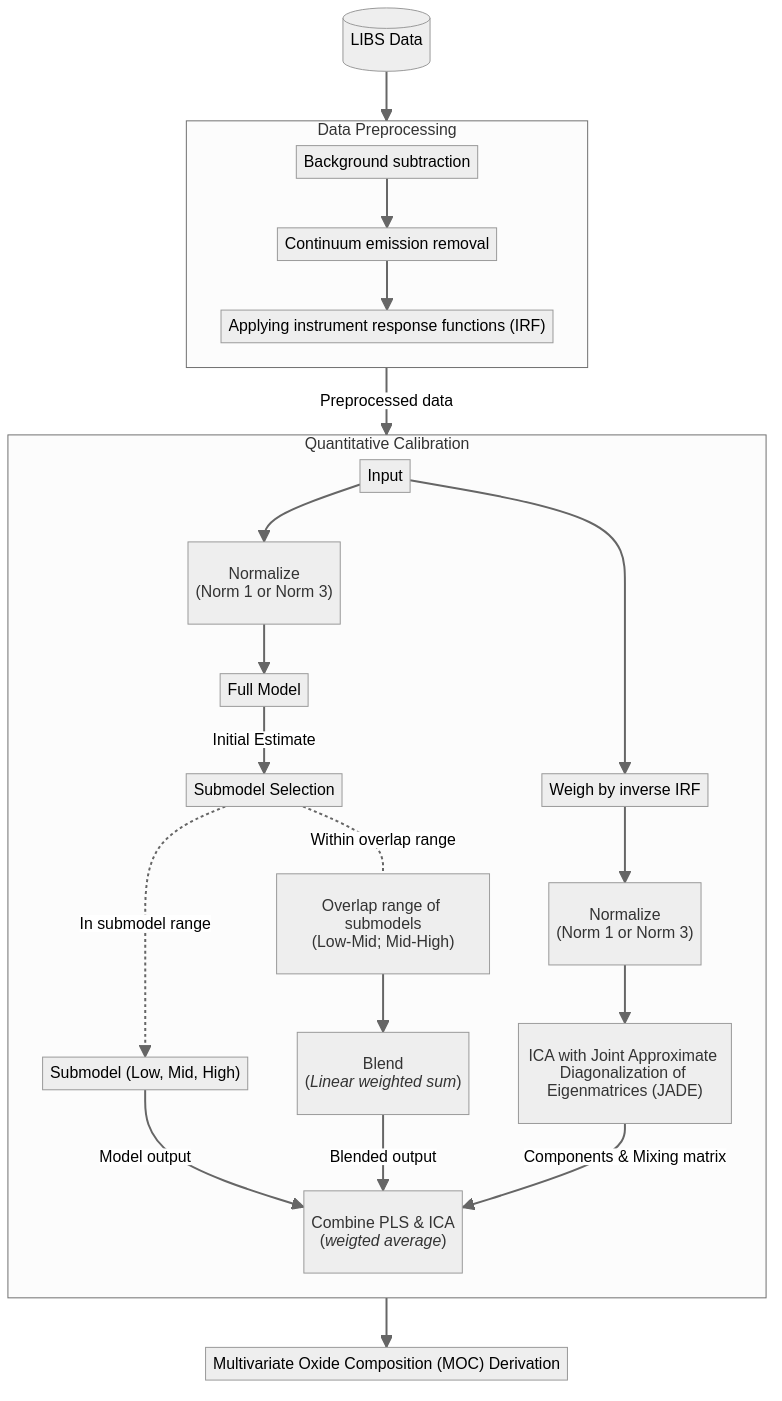
\includegraphics[width=0.45\textwidth]{images/pipeline.png}
    \caption{Flowchart illustrating MOC derivation via the ChemCam team's MOC model: data processing and calibration steps given LIBS data.}
    \label{fig:libs_data_processing}
\end{figure}

In Figure \ref{fig:libs_data_processing} we illustrate the data processing and calibration steps for LIBS data leading to the derivation of Multivariate Oxide Composition (MOC). The MOC model is described in details by \citet{cleggRecalibrationMarsScience2017} and \citet{andersonImprovedAccuracyQuantitative2017}, but we provide a brief overview here, which will serve as a foundation for the subsequent discussion of our work.

\subsubsection{Data Preprocessing}\label{sec:data_preprocessing}

The resulting data format is referred to as cleaned and calibrated spectra (CCS), which serves as the input for the system.
This format is a table of intensity values for each wavelength, with each row representing the intensities for a given shot, which is a single laser pulse on the sample, at that particular wavelength. An example of this data format is shown in Table~\ref{tab:example_data}. There are $6144$ rows and $N$ columns, where $N$ is the number of shots taken for a given sample. The number of shots taken for each sample can vary, but is typically between $15$ and $50$.

\begin{table}[ht]
\centering
\caption{Exemplary Data of Wavelengths and Shots}
\label{tab:example_data}
\begin{tabular}{|c|c|c|c|c|c|c|c|c|}
\hline
Wavelength & Shot 1   & Shot 2 & \ldots & Shot 50  \\ \hline
240.81     & 6.40e+15 & 4.04e+15 & \ldots& 1.75e+15 \\ \hline
240.86     & 3.85e+12 & 2.29e+12& \ldots & 7.28e+11 \\ \hline
\ldots     & \ldots & \ldots & \ldots & \ldots \\ \hline
905.38     & 1.88e+8 & 5.85e+7 & \ldots & 5.21e+9 \\ \hline
905.57     & 1.98e+10 & 1.29e+10& \ldots & 1.22e+10 \\ \hline
\end{tabular}
\end{table}



\subsubsection{Multivariate Oxide Composition Derivation}\label{sec:moc_derivation}

The multivariate analysis employs a composite approach integrating partial least squares regression with submodels (PLS-SM) and independent component analysis (ICA) to derive the Multivariate Oxide Composition (MOC).
The PLS-SM approach utilizes tailored sub-models for distinct composition ranges, enhancing accuracy at the boundaries of these ranges.
Independent Component Analysis assists in distinguishing elemental emission lines, contributing to a refined multivariate model.

Two normalization methods are employed in the analysis: Norm 1 and Norm 3.
Norm 1 standardizes the full spectrum across all three spectrometers such that the sum total is unity.
In contrast, Norm 3 conducts normalization on a per-spectrometer basis, culminating in a full normalized spectrum summing to three.
The optimal normalization technique is selected based on its efficacy in model performance for the specific analysis task at hand.

\subsubsection{Outlier Removal}\label{sec:outlier_removal}

In their analysis, \citet{andersonImprovedAccuracyQuantitative2017} employed a methodical outlier removal process to enhance model accuracy in multivariate regression. To detect outliers, they utilized influence plots, employing statistical measures that reflect each data point's deviation from the model's predictions and their influence on the model due to their position in the predictor space. 
In this context, the deviation, or the error, are known as residuals and the influence a data point has on the model is known as leverage.
The application of the following equation to latent variables enables the computation of an observation leverages vector (\(h_t\)):

\begin{equation}
    h_t = \text{diag}\left[ t(t^T t)^{-1} t^T \right]
\end{equation}

Where $t$ represents the PLS scores.
Given that leverage quantifies the distance of each observation from the model's center, it can be interpreted as the square Mahalanobis distance — a measure of the distance of a point from the center of mass of points in multivariate space. 
If the original data follows a multivariate normal distribution, the distances form a chi-squared distribution. Using this property, outliers can be detected using the chi-square test \cite{brereton_chi_2015}.
The Mahalanobis distance is defined as follows:

\begin{equation}
    D_M(p)^2 = (p - \mu)^T \cdot \Sigma^{-1} (p - \mu)
\end{equation}

Where $p$ is the point in question, $\mu$ is the mean of the distribution and $\Sigma^{-1}$ is the inverse of the covariance matrix of the distribution, known as the precision matrix. 
Variables exhibiting a high leverage score are indicative of predictors that deviate more significantly from the others, thereby have a greater influence on the model.
The measure of model fit, denoted as $Q$, is calculated by squaring the differences between the actual spectrum $x$ and the spectrum predicted by the model. This prediction uses the model's scores $t$ and loadings ($P$) to calculate the residuals $e$:

\begin{equation}
    e = x - t \cdot P^T
\end{equation}

The fit of model for the $i$th observation is then computed by taking the residual vector $e_i$ and multiplying it by the transpose of itself $e^T$, which gives you the sum of squared differences: 

\begin{equation}
    Q_i = e_{i}e_{i}^T
\end{equation} \cite{marini_chemometrics_2013} \citet{andersonImprovedAccuracyQuantitative2017}

Outlier removal is performed iteratively; an initial PLS model is conceived with cross-validation to determine the optimum number of latent variables, followed by an inspection of the influence plot to pinpoint outliers. Identified outliers are removed, and the model is re-evaluated. This procedure is repeated as needed, ensuring that any removals do not degrade the model's general performance.


\subsubsection{Partial Least Squares Sub-Models}\label{sec:pls_submodels}

\citet{andersonImprovedAccuracyQuantitative2017} proposed an approach referred to as the Partial Least Squares Sub-Models (PLS1-SM).
The inherent variability of LIBS spectral responses to different element concentrations necessitates a nuanced analysis. High element concentrations tend to obscure the spectral signal, and the presence of other elements further complicates the spectral response. A single regression model typically falls short in accounting for such variations, leading to compromises in predictive precision for specific samples.

They deployed multiple regression models, each tailored to subsets of the entire composition range, targeting "low," "mid," and "high" concentrations along with a comprehensive "full model." This led to the formation of 32 distinct models, with selected sub-model ranges that prioritize both a robust dataset and precise compositional response.

Each sub-model was subjected to training, cross-validation, and optimization phases, which included the iterative outlier removal strategy mentioned in section~\ref{sec:outlier_removal}. The full model's preliminary composition estimation of unknown targets dictates the choice of subsequent sub-model(s) for refined prediction.

PLS1-SM blends predictions from sub-models with overlapping concentration ranges. The predictions are linearly combined for a cohesive prediction. The full model projection $y_{\text{full}}$, if within a blend-ready range, determines the final prediction $y_{\text{final}}$ through a weighted sum of overlapping sub-model predictions:

\begin{align*}
w_{\text{mid}} &= \frac{y_{\text{full}}-y_{\text{blend range, min}}}{y_{\text{blend range, max}} - y_{\text{blend range, min}}} \\
w_{\text{low}} &= 1 - w_{\text{mid}} \\
y_{\text{final}} &= w_{\text{low}}\cdot y_{\text{low}} + w_{\text{mid}}\cdot y_{\text{mid}} 
\end{align*}

This applies analogously for predictions in the "mid-high" range to prevent prediction discontinuities.

The exact delineations of the blending ranges are adjustable, with optimization performed using the Broyden-Fletcher-Goldfarb-Shannon (BFGS) algorithm. This process, aimed at minimizing the RMSE for the full model dataset, established optimal ranges. Initial blend boundaries were predicated on sub-model intersections, with exceptional outliers managed distinctly due to their deviation from expected value ranges.

\subsubsection{Independent Component Analysis}\label{sec:ica}
\citet{cleggRecalibrationMarsScience2017} and \cite{forniIndependentComponentAnalysis2013} proposed the use of Independent Component Analysis (ICA) to identify the elemental emission lines in LIBS spectra. Independent Component Analysis (ICA) is a computational method used to separate a multivariate signal into additive, statistically independent components, particularly useful in scenarios where the signal sources overlap, such as in LIBS data.

ICA yields independent source components and the affiliated mixing matrix which illustrates how the independent sources are combined to form the observed spectral data.

After extracting the independent components, the key task is to associate each independent component with a specific elemental emission line. 
This process involves examining the emission lines of the elements and evaluating the ICA scores. 
These scores reflect the correlation between each Independent Component and the entire spectrum of wavelengths. 
Subsequently, these correlation values (ICA scores) are employed to establish a calibration curve, which correlates the ICA score to the elemental composition.

To ascertain the accuracy of this calibration, a regression analysis is performed using multiple regression functions. The function that provides the most reliable fit (often assessed through chi-square values) is used to predict the composition for each element.

Model refinement is facilitated by techniques such as normalization, outlier removal (via Median Absolute Deviation), and k-fold cross-validation. These methods ensure the robustness and reliability of the predictive model constructed through ICA.